\documentclass[12pt,letterpaper]{article}
\usepackage{graphicx,textcomp}
\usepackage{natbib}
\usepackage{setspace}
\usepackage{fullpage}
\usepackage{color}
\usepackage[reqno]{amsmath}
\usepackage{amsthm}
\usepackage{fancyvrb}
\usepackage{amssymb,enumerate}
\usepackage[all]{xy}
\usepackage{endnotes}
\usepackage{lscape}
\newtheorem{com}{Comment}
\usepackage{float}
\usepackage{hyperref}
\newtheorem{lem} {Lemma}
\newtheorem{prop}{Proposition}
\newtheorem{thm}{Theorem}
\newtheorem{defn}{Definition}
\newtheorem{cor}{Corollary}
\newtheorem{obs}{Observation}
\usepackage[compact]{titlesec}
\usepackage{dcolumn}
\usepackage{tikz}
\usetikzlibrary{arrows}
\usepackage{multirow}
\usepackage{xcolor}
\newcolumntype{.}{D{.}{.}{-1}}
\newcolumntype{d}[1]{D{.}{.}{#1}}
\definecolor{light-gray}{gray}{0.65}
\usepackage{url}
\usepackage{listings}
\usepackage{color}

\definecolor{codegreen}{rgb}{0,0.6,0}
\definecolor{codegray}{rgb}{0.5,0.5,0.5}
\definecolor{codepurple}{rgb}{0.58,0,0.82}
\definecolor{backcolour}{rgb}{0.95,0.95,0.92}

\lstdefinestyle{mystyle}{
	backgroundcolor=\color{backcolour},   
	commentstyle=\color{codegreen},
	keywordstyle=\color{magenta},
	numberstyle=\tiny\color{codegray},
	stringstyle=\color{codepurple},
	basicstyle=\footnotesize,
	breakatwhitespace=false,         
	breaklines=true,                 
	captionpos=b,                    
	keepspaces=true,                 
	numbers=left,                    
	numbersep=5pt,                  
	showspaces=false,                
	showstringspaces=false,
	showtabs=false,                  
	tabsize=2
}
\lstset{style=mystyle}
\newcommand{\Sref}[1]{Section~\ref{#1}}
\newtheorem{hyp}{Hypothesis}

\title{Problem Set 2}
\date{Due: October 15, 2023}
\author{Liu Yuanyuan}

\begin{document}
	\maketitle
	\section*{Instructions}
\begin{itemize}
	\item Please show your work! You may lose points by simply writing in the answer. If the problem requires you to execute commands in \texttt{R}, please include the code you used to get your answers. Please also include the \texttt{.R} file that contains your code. If you are not sure if work needs to be shown for a particular problem, please ask.
	\item Your homework should be submitted electronically on GitHub.
	\item This problem set is due before 23:59 on Sunday October 15, 2023. No late assignments will be accepted.

\end{itemize}

	
	\vspace{.5cm}
	\section*{Question 1: Political Science}
		\vspace{.25cm}
	The following table was created using the data from a study run in a major Latin American city.\footnote{Fried, Lagunes, and Venkataramani (2010). ``Corruption and Inequality at the Crossroad: A Multimethod Study of Bribery and Discrimination in Latin America. \textit{Latin American Research Review}. 45 (1): 76-97.} As part of the experimental treatment in the study, one employee of the research team was chosen to make illegal left turns across traffic to draw the attention of the police officers on shift. Two employee drivers were upper class, two were lower class drivers, and the identity of the driver was randomly assigned per encounter. The researchers were interested in whether officers were more or less likely to solicit a bribe from drivers depending on their class (officers use phrases like, ``We can solve this the easy way'' to draw a bribe). The table below shows the resulting data.

\newpage
\begin{table}[h!]
	\centering
	\begin{tabular}{l | c c c }
		& Not Stopped & Bribe requested & Stopped/given warning \\
		\\[-1.8ex] 
		\hline \\[-1.8ex]
		Upper class & 14 & 6 & 7 \\
		Lower class & 7 & 7 & 1 \\
		\hline
	\end{tabular}
\end{table}

\begin{enumerate}
	
	\item [(a)]
	Calculate the $\chi^2$ test statistic by hand/manually (even better if you can do "by hand" in \texttt{R}).\\
	\lstinputlisting[language=R,firstline=2,lastline=20]{PS02_Yuanyuan_Liu.R}
    \begin{itemize}
    \item \textbf{Result}:\\
    the $\chi^2$ test statistic is:3.791168
    \end{itemize}

	
	\item [(b)]
	Now calculate the p-value from the test statistic you just created (in \texttt{R}).\footnote{Remember frequency should be $>$ 5 for all cells, but let's calculate the p-value here anyway.}  What do you conclude if $\alpha = 0.1$?\\
		\lstinputlisting[language=R,firstline=23,lastline=30]{PS02_Yuanyuan_Liu.R}
	\begin{itemize}
		\item \textbf{Result}:\\
		p-value:0.1502306\\
		under the significance level a=0.1,we fail to reject null hypothesis,the officer were less likely to solicit a bribe from drivers depending on their class.
	\end{itemize}
	
	\item [(c)] Calculate the standardized residuals for each cell and put them in the table below.
	\vspace{1cm}
		\lstinputlisting[language=R,firstline=33,lastline=40]{PS02_Yuanyuan_Liu.R}
	\begin{table}[h]
		\centering
		\begin{tabular}{l | c c c }
			& Not Stopped & Bribe requested & Stopped/given warning \\
			\\[-1.8ex] 
			\hline \\[-1.8ex]
			Upper class  & 0.02430 &-0.23574 &  0.20195 \\
			\\
			Lower class &-0.08104 &0.35162 & -0.57177  \\
			
		\end{tabular}
	\end{table}
	
	
	\vspace{1cm}
	\item [(d)] How might the standardized residuals help you interpret the results?  
	\begin{itemize}
	\item \textbf{Result}:\\
	under the significance level a=0.1,we fail to reject null hypothesis,the officer were less likely to solicit a bribe from drivers depending on their class.For data with positive standardized residuals, which indicates that the observed frequency is higher than the predetermined frequency, positive residual standard deviations indicate that police are more likely to obtain tickets from these drivers. For data with negative standardized residuals, this means that the observed frequency is lower than the predetermined frequency, in which case a negative residual means that the police are less likely to obtain tickets from these drivers. Based on the above data, the social class of drivers may have an impact on bribery behavior between police and drivers. Police are more likely to demand bribes from drivers of higher social class.
   \end{itemize}
	
\end{enumerate}
\newpage

\section*{Question 2: Economics}
Chattopadhyay and Duflo were interested in whether women promote different policies than men.\footnote{Chattopadhyay and Duflo. (2004). ``Women as Policy Makers: Evidence from a Randomized Policy Experiment in India. \textit{Econometrica}. 72 (5), 1409-1443.} Answering this question with observational data is pretty difficult due to potential confounding problems (e.g. the districts that choose female politicians are likely to systematically differ in other aspects too). Hence, they exploit a randomized policy experiment in India, where since the mid-1990s, $\frac{1}{3}$ of village council heads have been randomly reserved for women. A subset of the data from West Bengal can be found at the following link: \url{https://raw.githubusercontent.com/kosukeimai/qss/master/PREDICTION/women.csv}\\

\noindent Each observation in the data set represents a village and there are two villages associated with one GP (i.e. a level of government is called "GP"). Figure~\ref{fig:women_desc} below shows the names and descriptions of the variables in the dataset. The authors hypothesize that female politicians are more likely to support policies female voters want. Researchers found that more women complain about the quality of drinking water than men. You need to estimate the effect of the reservation policy on the number of new or repaired drinking water facilities in the villages.
\vspace{.5cm}
\begin{figure}[h!]
	\caption{\footnotesize{Names and description of variables from Chattopadhyay and Duflo (2004).}}
	\vspace{.5cm}
	\centering
	\label{fig:women_desc}
	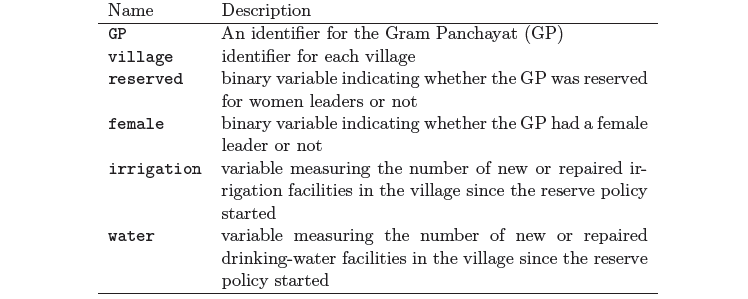
\includegraphics[width=1.1\textwidth]{women_desc.png}
\end{figure}		

\newpage
\begin{enumerate}
	\item [(a)] State a null and alternative (two-tailed) hypothesis. 
	\begin{itemize}
		\item \textbf{Result}:\\
	H0:The reservation policy has no effect on the number of new or repaired drinking water facilities in the villages\\
	H1:The reservation policy has effect on the number of new or repaired drinking water facilities in the villages
	\end{itemize}
	\vspace{1cm}
	\item [(b)] Run a bivariate regression to test this hypothesis in \texttt{R} (include your code!).
		\lstinputlisting[language=R,firstline=52,lastline=57]{PS02_Yuanyuan_Liu.R}
	\begin{itemize}
		\item \textbf{Result}:\\
		Call:
		lm(formula = Y ~ X)
		 
		Residuals:
		           
		   
			\begin{table}[h]
			\centering
			\begin{tabular}{l | c c c c c}
				& Min   & 1Q  r &Median   & 3Q  &Max   \\
				\\[-1.8ex] 
				\hline \\[-1.8ex]
				  & -23.991&-14.738  &  -7.865   &2.262 &316.009 \\
				                                 
			\end{tabular}
		\end{table}
		Coefficients: 
			\begin{table}[h]
			\centering
			\begin{tabular}{l | c c c c }
				& Estimate & Std. Error & t &  Pr(>|t|) \\
				\\[-1.8ex] 
				\hline \\[-1.8ex]
			(Intercept)  & 14.738 & 2.286  &  6.446 &4.22e-10  \\
				\\
				X  &9.252 & 3.948  & 2.344 & 0.0197\\
				
			\end{tabular}
		\end{table}

		Signif. codes:  
		0 ‘***’ 0.001 ‘**’ 0.01 ‘*’ 0.05 ‘.’ 0.1 ‘ ’ 1
		
		Residual standard error: 33.45 on 320 degrees of freedom\\
		Multiple R-squared:  0.01688,	Adjusted R-squared:  0.0138 \\
		F-statistic: 5.493 on 1 and 320 DF,  p-value: 0.0197
		
	\end{itemize}
	
	
	\vspace{1cm}
	\item [(c)] Interpret the coefficient estimate for reservation policy. 
		\begin{itemize}
		\item \textbf{Result}:\\
		1.Intercept: It represents the predicted value of the explained variable when the explanatory variable is equal to zero. When the reservation policy is equal to zero, the value of the number of new or repaired drinking water facilities in the villages approximately is 14.738.\\
		2.Slop:The coefficient of X is estimated to be positive, indicating that there is a positive correlation between the  increase of new water or repaired drinking water facilities in the villages and reservation. with the increase per unit of reservation, the number of new water or repaired drinking water facilities in the villages will increase by 9.252\\
		3.Std.Error:Standard Error is an estimate of the standard deviation of the regression coefficient estimate in regression analysis. It measures the uncertainty or variability in the coefficient estimates in a regression model. I this model, the estimate of X is 2.344, indicates a more precise estimate of the coefficient.\\
		4.t-value and p-value: t-value and p-value are used to measure the significance of the coefficient estimates. In this model, the t-value of the reservation variable is 2.344, the p-value is 0.0197. That means on the confidence interval of 0.05, we can reject H0, the reservation policy has a significant effect on the number of new or repaired drinking water facilities in the villages.The p-value of intercept is 4.22e-10,is approximately equal to zero, there is sufficient evidence to conclude that the intercept differs significantly from zero\\
		
	\end{itemize}
\end{enumerate}

\end{document}
